\subsection{Lectura}

Se implementó la funcionalidad en el software SettDev para leer y reproducir un archivo. La Figura \ref{fig:cargaarchivo} muestra el módulo de carga de un archivo. El programa permite abrir un cuadro de diálogo para seleccionar un archivo del equipo, de tipo .bin. Cuando se da clic al botón ``Abrir'' y se cierra el archivo, el programa verifica la extensión del archivo. Posteriormente, comienza a leer los datos del archivo.

\begin{figure}[htb]
	\centering
	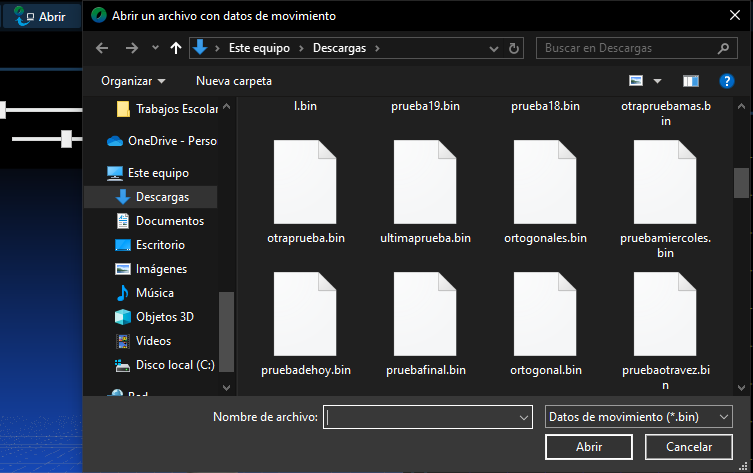
\includegraphics[scale=0.65]{cargaarchivo.png}
	\caption{Módulo de carga de archivo implementado en SettDev}
	\label{fig:cargaarchivo}
\end{figure}